\documentclass[14pt]{extbook}
\usepackage{multicol, enumerate, enumitem, hyperref, color, soul, setspace, parskip, fancyhdr} %General Packages
\usepackage{amssymb, amsthm, amsmath, latexsym, units, mathtools} %Math Packages
\everymath{\displaystyle} %All math in Display Style
% Packages with additional options
\usepackage[headsep=0.5cm,headheight=12pt, left=1 in,right= 1 in,top= 1 in,bottom= 1 in]{geometry}
\usepackage[usenames,dvipsnames]{xcolor}
\usepackage{dashrule}  % Package to use the command below to create lines between items
\newcommand{\litem}[1]{\item#1\hspace*{-1cm}\rule{\textwidth}{0.4pt}}
\pagestyle{fancy}
\lhead{Progress Quiz 6}
\chead{}
\rhead{Version B}
\lfoot{1430-1829}
\cfoot{}
\rfoot{test}
\begin{document}

\begin{enumerate}
\litem{
Write the equation of the graph presented below in the form $f(x)=ax^2+bx+c$, assuming  $a=1$ or $a=-1$. Then, choose the intervals that $a, b,$ and $c$ belong to.
\begin{center}
    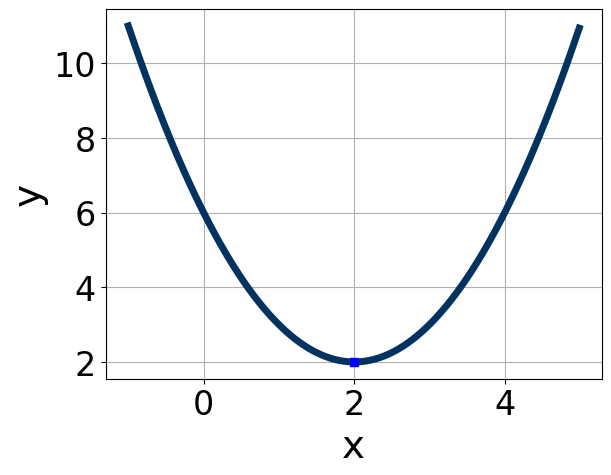
\includegraphics[width=0.5\textwidth]{../Figures/quadraticGraphToEquationCopyB.png}
\end{center}
\begin{enumerate}[label=\Alph*.]
\item \( a \in [0.6, 1.4], \hspace*{5mm} b \in [4, 5], \text{ and } \hspace*{5mm} c \in [-9, -5] \)
\item \( a \in [0.6, 1.4], \hspace*{5mm} b \in [-4, -1], \text{ and } \hspace*{5mm} c \in [-9, -5] \)
\item \( a \in [0.6, 1.4], \hspace*{5mm} b \in [-4, -1], \text{ and } \hspace*{5mm} c \in [13, 18] \)
\item \( a \in [-2.9, 0.6], \hspace*{5mm} b \in [-4, -1], \text{ and } \hspace*{5mm} c \in [-16, -9] \)
\item \( a \in [-2.9, 0.6], \hspace*{5mm} b \in [4, 5], \text{ and } \hspace*{5mm} c \in [-16, -9] \)

\end{enumerate} }
\litem{
Factor the quadratic below. Then, choose the intervals that contain the constants in the form $(ax+b)(cx+d); b \leq d.$\[ 36x^{2} +60 x + 25 \]\begin{enumerate}[label=\Alph*.]
\item \( a \in [1.26, 2.42], \hspace*{5mm} b \in [5, 6], \hspace*{5mm} c \in [14.8, 22], \text{ and } \hspace*{5mm} d \in [2, 13] \)
\item \( a \in [5.78, 7.46], \hspace*{5mm} b \in [5, 6], \hspace*{5mm} c \in [3.4, 7.2], \text{ and } \hspace*{5mm} d \in [2, 13] \)
\item \( a \in [0.34, 1.84], \hspace*{5mm} b \in [24, 31], \hspace*{5mm} c \in [0, 2.4], \text{ and } \hspace*{5mm} d \in [30, 38] \)
\item \( a \in [11.81, 12.31], \hspace*{5mm} b \in [5, 6], \hspace*{5mm} c \in [1.9, 4], \text{ and } \hspace*{5mm} d \in [2, 13] \)
\item \( \text{None of the above.} \)

\end{enumerate} }
\litem{
Solve the quadratic equation below. Then, choose the intervals that the solutions $x_1$ and $x_2$ belong to, with $x_1 \leq x_2$.\[ 10x^{2} -57 x + 54 = 0 \]\begin{enumerate}[label=\Alph*.]
\item \( x_1 \in [1.16, 1.43] \text{ and } x_2 \in [4.48, 5.26] \)
\item \( x_1 \in [1.37, 1.57] \text{ and } x_2 \in [3.19, 3.99] \)
\item \( x_1 \in [-0.08, 0.49] \text{ and } x_2 \in [13.28, 14.09] \)
\item \( x_1 \in [0.87, 1.18] \text{ and } x_2 \in [5.98, 6.39] \)
\item \( x_1 \in [11.77, 12.1] \text{ and } x_2 \in [44.4, 45.03] \)

\end{enumerate} }
\litem{
Graph the equation below.\[ f(x) = -(x+3)^2 - 13 \]\begin{enumerate}[label=\Alph*.]
\begin{multicols}{2}\item 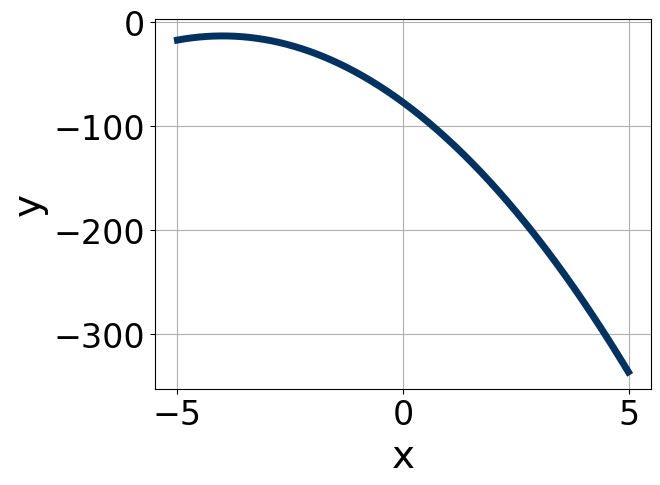
\includegraphics[width = 0.3\textwidth]{../Figures/quadraticEquationToGraphCopyAB.png}\item 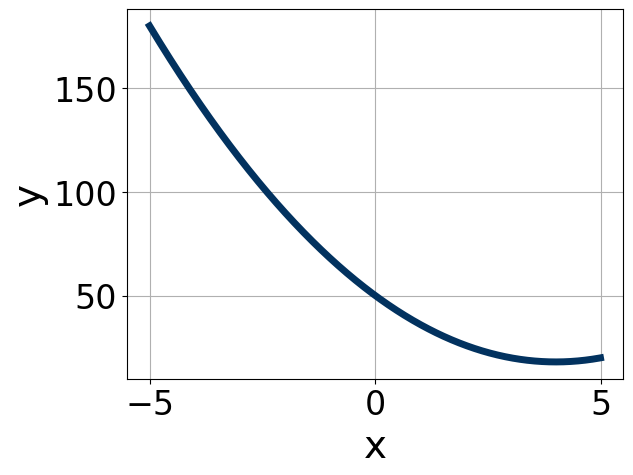
\includegraphics[width = 0.3\textwidth]{../Figures/quadraticEquationToGraphCopyBB.png}\item 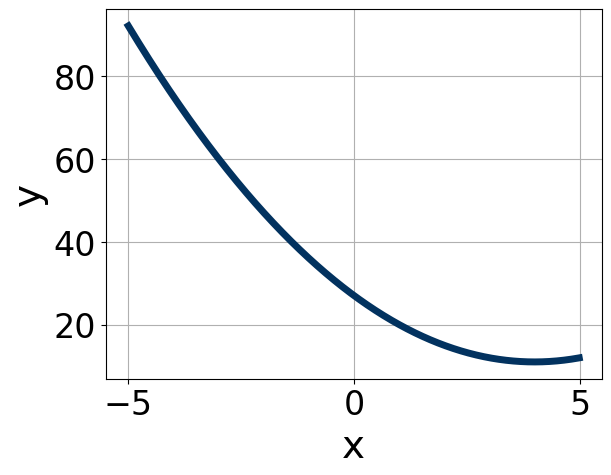
\includegraphics[width = 0.3\textwidth]{../Figures/quadraticEquationToGraphCopyCB.png}\item 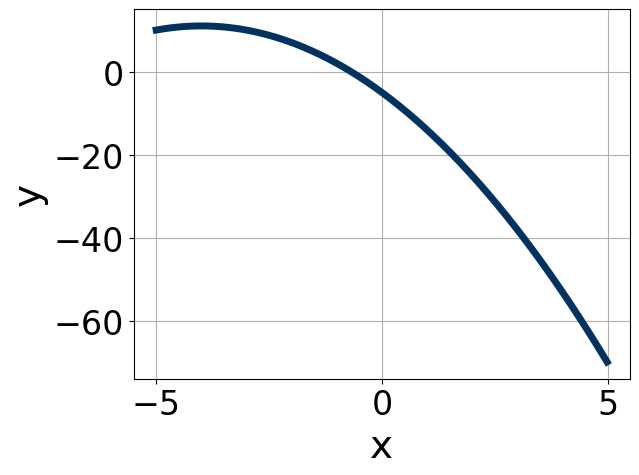
\includegraphics[width = 0.3\textwidth]{../Figures/quadraticEquationToGraphCopyDB.png}\end{multicols}\item None of the above.
\end{enumerate} }
\litem{
Graph the equation below.\[ f(x) = -(x-2)^2 + 19 \]\begin{enumerate}[label=\Alph*.]
\begin{multicols}{2}\item 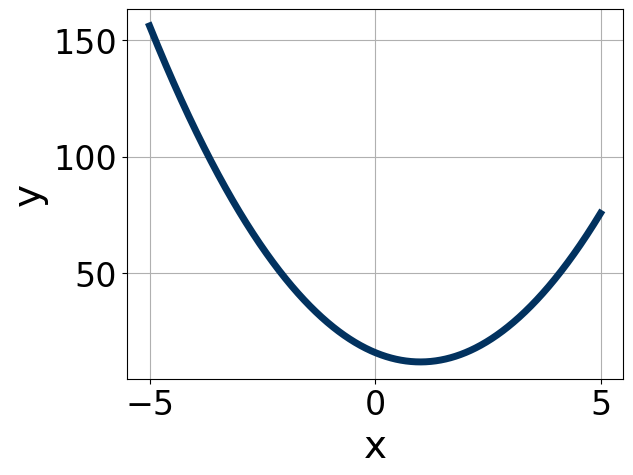
\includegraphics[width = 0.3\textwidth]{../Figures/quadraticEquationToGraphAB.png}\item 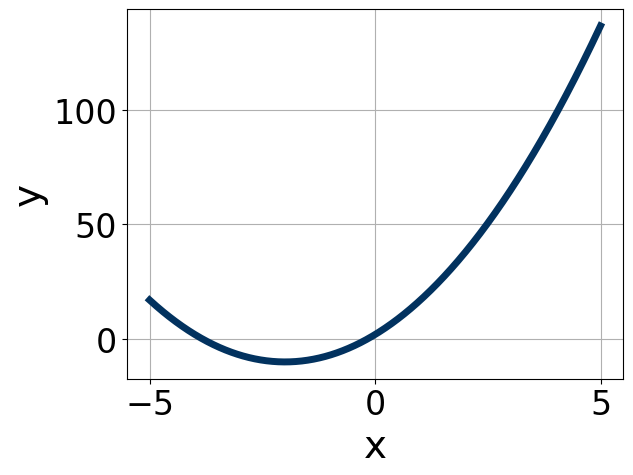
\includegraphics[width = 0.3\textwidth]{../Figures/quadraticEquationToGraphBB.png}\item 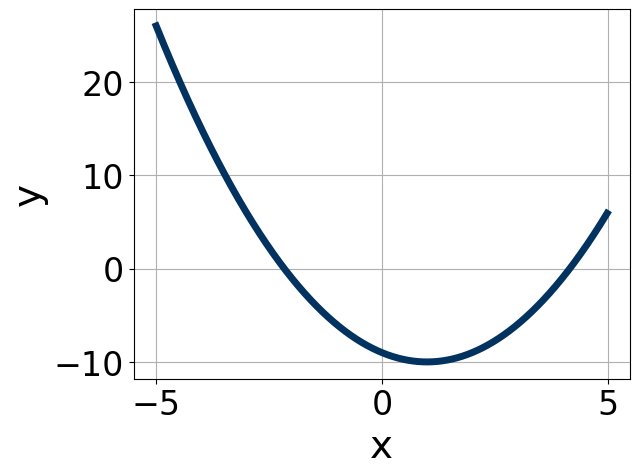
\includegraphics[width = 0.3\textwidth]{../Figures/quadraticEquationToGraphCB.png}\item 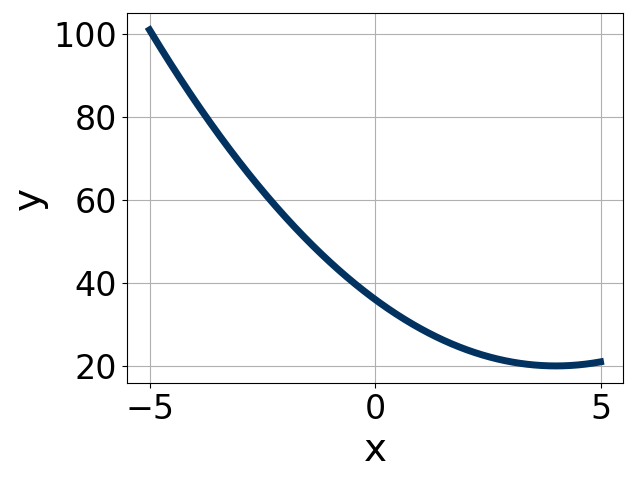
\includegraphics[width = 0.3\textwidth]{../Figures/quadraticEquationToGraphDB.png}\end{multicols}\item None of the above.
\end{enumerate} }
\litem{
Write the equation of the graph presented below in the form $f(x)=ax^2+bx+c$, assuming  $a=1$ or $a=-1$. Then, choose the intervals that $a, b,$ and $c$ belong to.
\begin{center}
    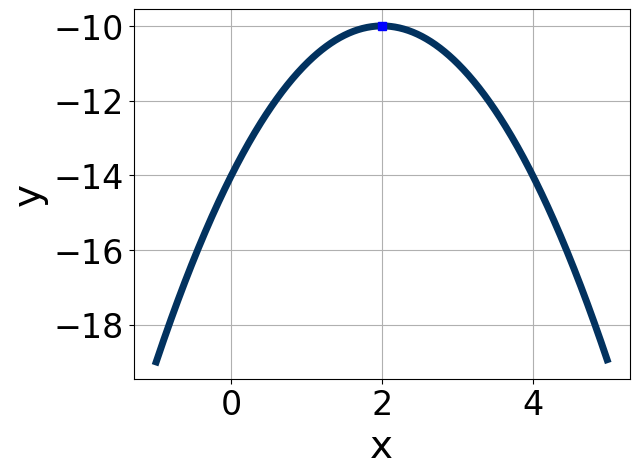
\includegraphics[width=0.5\textwidth]{../Figures/quadraticGraphToEquationB.png}
\end{center}
\begin{enumerate}[label=\Alph*.]
\item \( a \in [-2, 0], \hspace*{5mm} b \in [-5, -3], \text{ and } \hspace*{5mm} c \in [3, 8] \)
\item \( a \in [-2, 0], \hspace*{5mm} b \in [1, 5], \text{ and } \hspace*{5mm} c \in [-15, -11] \)
\item \( a \in [-0.5, 1.2], \hspace*{5mm} b \in [1, 5], \text{ and } \hspace*{5mm} c \in [14, 18] \)
\item \( a \in [-0.5, 1.2], \hspace*{5mm} b \in [-5, -3], \text{ and } \hspace*{5mm} c \in [14, 18] \)
\item \( a \in [-2, 0], \hspace*{5mm} b \in [1, 5], \text{ and } \hspace*{5mm} c \in [3, 8] \)

\end{enumerate} }
\litem{
Solve the quadratic equation below. Then, choose the intervals that the solutions $x_1$ and $x_2$ belong to, with $x_1 \leq x_2$.\[ 10x^{2} +57 x + 54 = 0 \]\begin{enumerate}[label=\Alph*.]
\item \( x_1 \in [-12.3, -8.5] \text{ and } x_2 \in [-0.64, -0.58] \)
\item \( x_1 \in [-45.7, -42.8] \text{ and } x_2 \in [-12.01, -11.48] \)
\item \( x_1 \in [-16.5, -13.3] \text{ and } x_2 \in [-0.55, -0.36] \)
\item \( x_1 \in [-6.5, -2.9] \text{ and } x_2 \in [-1.39, -1.17] \)
\item \( x_1 \in [-3.1, -0.2] \text{ and } x_2 \in [-2.29, -2.04] \)

\end{enumerate} }
\litem{
Factor the quadratic below. Then, choose the intervals that contain the constants in the form $(ax+b)(cx+d); b \leq d.$\[ 24x^{2} +2 x -15 \]\begin{enumerate}[label=\Alph*.]
\item \( a \in [1.72, 2.18], \hspace*{5mm} b \in [-4, 5], \hspace*{5mm} c \in [10.1, 12.1], \text{ and } \hspace*{5mm} d \in [0, 7] \)
\item \( a \in [3.56, 4.04], \hspace*{5mm} b \in [-4, 5], \hspace*{5mm} c \in [4.1, 8.7], \text{ and } \hspace*{5mm} d \in [0, 7] \)
\item \( a \in [0.92, 1.26], \hspace*{5mm} b \in [-19, -11], \hspace*{5mm} c \in [0.5, 1.4], \text{ and } \hspace*{5mm} d \in [18, 23] \)
\item \( a \in [7.74, 8.18], \hspace*{5mm} b \in [-4, 5], \hspace*{5mm} c \in [1.3, 5.8], \text{ and } \hspace*{5mm} d \in [0, 7] \)
\item \( \text{None of the above.} \)

\end{enumerate} }
\litem{
Solve the quadratic equation below. Then, choose the intervals that the solutions belong to, with $x_1 \leq x_2$ (if they exist).\[ 14x^{2} +7 x -4 = 0 \]\begin{enumerate}[label=\Alph*.]
\item \( x_1 \in [-17.5, -16.15] \text{ and } x_2 \in [15.1, 17.1] \)
\item \( x_1 \in [-0.8, 0.16] \text{ and } x_2 \in [0.5, 1.4] \)
\item \( x_1 \in [-11.88, -11.23] \text{ and } x_2 \in [4.7, 6.1] \)
\item \( x_1 \in [-2.17, -0.36] \text{ and } x_2 \in [-1.6, 0.8] \)
\item \( \text{There are no Real solutions.} \)

\end{enumerate} }
\litem{
Solve the quadratic equation below. Then, choose the intervals that the solutions belong to, with $x_1 \leq x_2$ (if they exist).\[ -15x^{2} -8 x + 6 = 0 \]\begin{enumerate}[label=\Alph*.]
\item \( x_1 \in [-6.6, -6.16] \text{ and } x_2 \in [13.6, 16] \)
\item \( x_1 \in [-1.19, -0.93] \text{ and } x_2 \in [-0.9, 0.8] \)
\item \( x_1 \in [-0.73, -0.03] \text{ and } x_2 \in [0.6, 2.6] \)
\item \( x_1 \in [-20.96, -20.58] \text{ and } x_2 \in [18.7, 20.4] \)
\item \( \text{There are no Real solutions.} \)

\end{enumerate} }
\end{enumerate}

\end{document}